\section{Resolving Ambiguities Using the Abstraction Tree}
\subsection{Resolving Context Ambiguities}
\begin{Verbatim}
Algorithm 1
function [HM]=eligible(HM_tree,Req)
BM = root of HM_tree
while (BM is not empty)
 For every model M in BM
  If (all behaviors in Prop(Req) are not abstracted with other behaviors)
   Remove M from BM
   save M in HM
  else
   add children of M in BM
  endif
 endfor
endwhile
Return HM
\end{Verbatim}
%BM = all models in HM_tree with all Prop(Req)
%For all M in BM
 %while (in the parent of M no behavior in Prop(Req) is abstracted with other behaviors)
	 %M = parent of M
 %endwhile
 %save M in HM
 %endfor
\subsection{Resolving Validity Ambiguities}

\begin{Verbatim}
Algorithm 2
Input: system model PM, abstraction tree for environment HM_tree, requirement Req
Output: Counter examples CE and corresponding model refinements
[HM]=eligible(HM_tree,Req);
Mc= HM;
 while (Mc is not empty)
  For all M in Mc
   [satisfied,CE]=ModelChecking(M,PM,Req);
	 Remove M from Mc
	 If satisfied==0
	  add the children of M to Mc
		cache CE
	else
		save CE from the parent model
	endif
 endfor
endwhile
Return all saved CEs and their corresponding models
\end{Verbatim}



\section{Case Study: Closed-loop Model Checking of a Dual Chamber Pacemaker}
\label{contextAmbiguities}
\subsection{Requirement Encoding}
\begin{itemize}
	\item Pre-condition: Atrial self-activation rate (60bpm - 150bpm)
    \item Post-condition: Intervals between ventricular paces should be no shorter than 500ms
\end{itemize}
\Hao{Need a monitor here}
The requirement can be translated to:
$$Req1: NA\_self.min=600 \&\& NA\_self.max=1000 \&\& M.state=check\Rightarrow M.t_m>=500$$
$Prop(Req1)=NA.self$
\subsection{Solving Requirement Ambiguities}
To verify the closed-loop system with pacemaker model $PM$ and heart model abstraction tree $HM\_tree$ (\figref{abs_exam}) against requirement $Req1$, we start by calling the function $[HM]=eligible(HM\_tree,Req1)$. In the root level heart model $H_{all}$, \emph{Rule 7} has been applied which abstract the $cond$ behavior of the path to the $self$ behavior of the nodes, including $NA.self$. As the result, the children of $H_{all}$ are examined and $NA.self$ is not abstracted with other behaviors in $H_n'',H_{at}'''',H_{vt}'''$. These 3 heart models are outputted as the appropriate models for $Req1$.
\subsection{Solving Validity Ambiguities}
After we choose the appropriate models for the requirement with 
$$HM=\{H_n'',H_{at}'''',H_{vt}'''\}$$
By model checking on all 3 initial models in UPPAAL we have: 
$$[1,[]]=ModelChecking(H_n'',PM,Req1)$$
 $$[0,CE_1]=ModelChecking(H_{at}'''',PM,Req1)$$
$$[0,CE_2]=ModelChecking(H_{vt}''',PM,Req1)$$
The algorithm keeps going down the abstraction tree, and at certain intermediate step we have:
 $$[0,CE_a]=ModelChecking(H_{st}',PM,Req1)$$
  $$[0,CE_b]=ModelChecking(H_{pvc}',PM,Req1)$$
	$$[0,CE_c]=ModelChecking(H_{at},PM,Req1)$$
 $$[1,[]]=ModelChecking(H_{vr}'',PM,Req1)$$
 $$[1,[]]=ModelChecking(H_{vf}'',PM,Req1)$$
The counter-examples are illustrated in \figref{CE}.
\begin{figure}[!t]
		\centering
		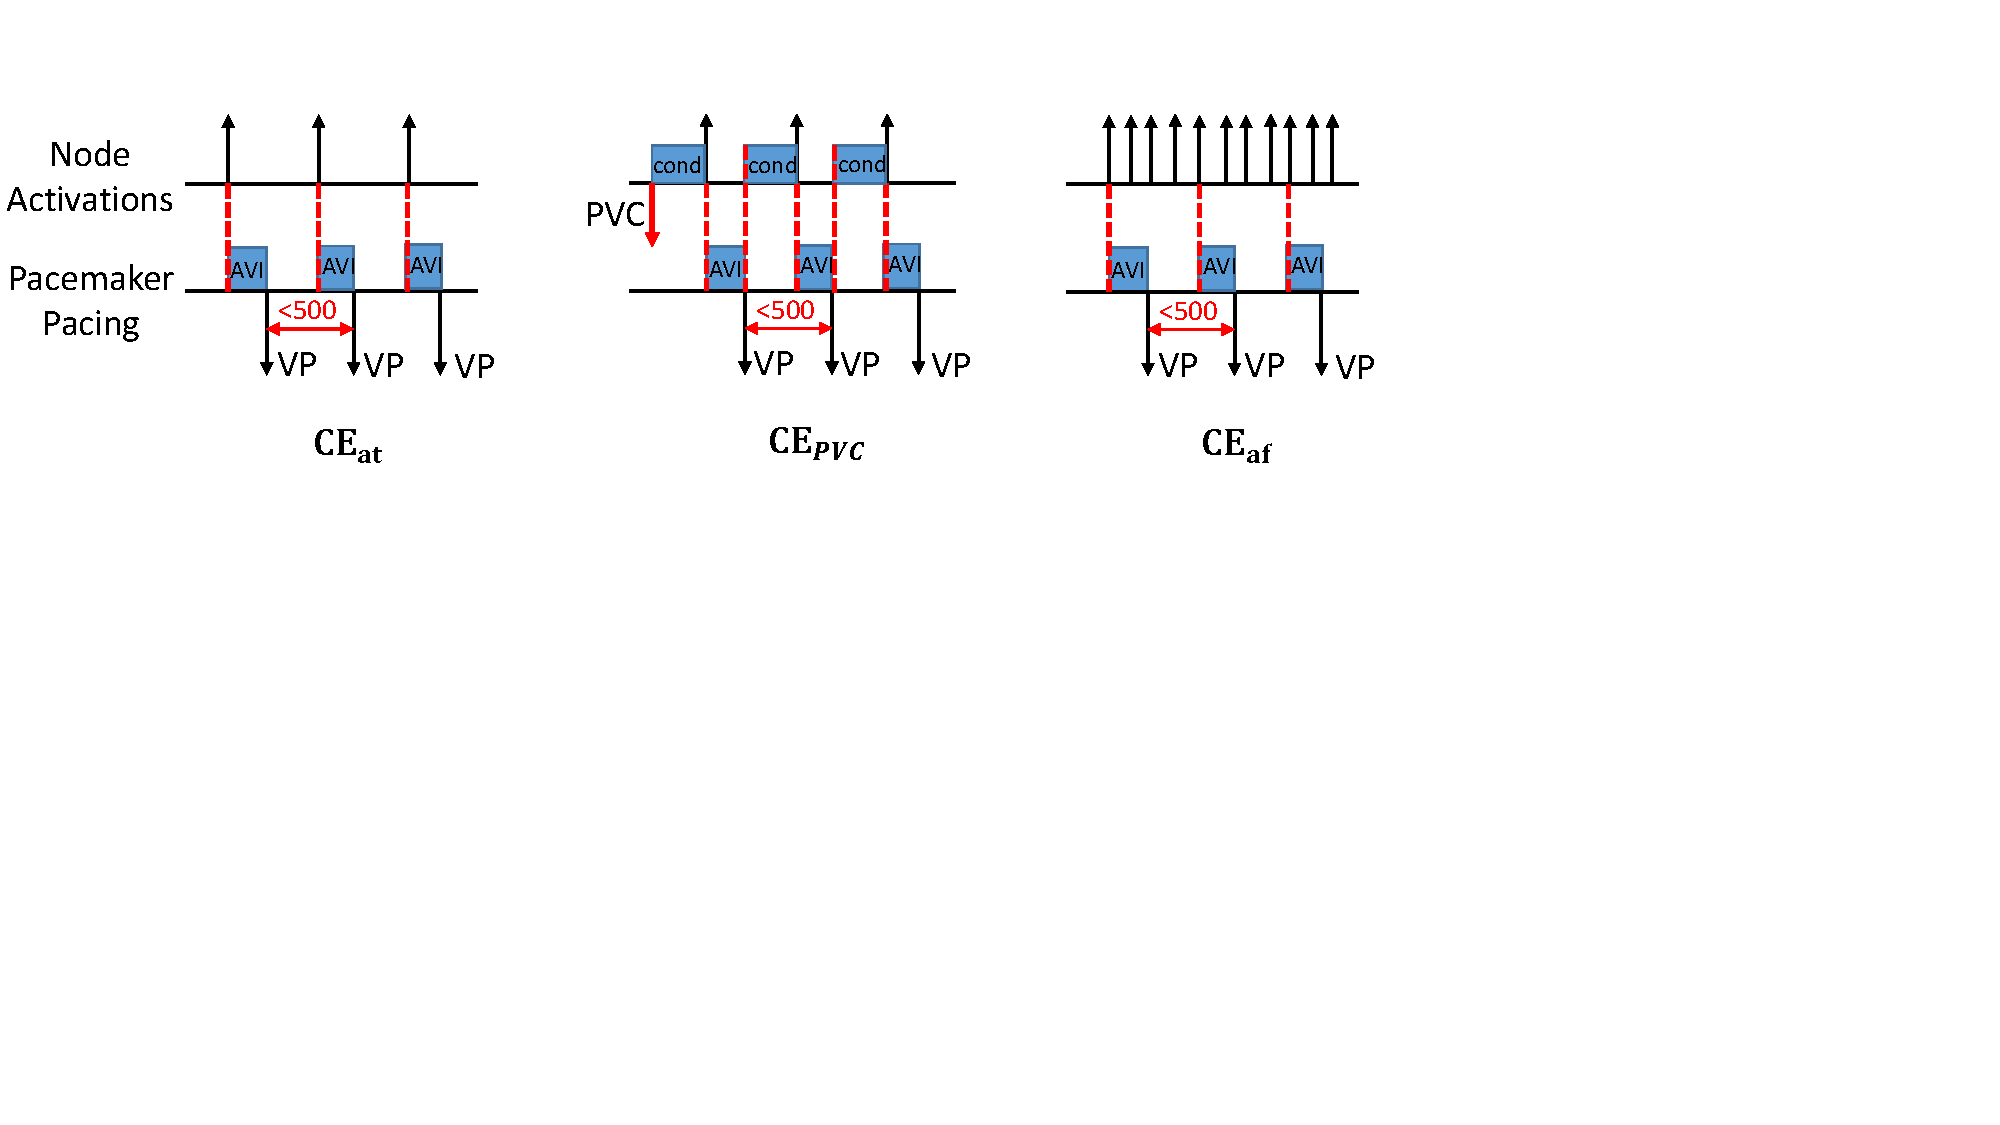
\includegraphics[width=0.9\textwidth]{figs/case.pdf}
		%\vspace{-5pt}
		\caption{\small Counter-examples}
		  %\vspace{-15pt}
		\label{fig:CE}
\end{figure}
$CE_a$ is a save execution of the pacemaker. $CE_b$ is Endless Loop Tachycardia. $CE_c$ is referred to as Atrial Tachycardia Response of a pacemaker. Both $CE_b$ and $CE_c$ are inappropriate executions of the pacemaker .$CE_a$ and $CE_b$ can have the same input-output executions on the pacemaker side and can only be differentiated on the heart model side. After the physician examines the counter-example the programmer can work on debugging.
%$NA\_self$ is in $H_3$, we go one level up, in $H_4$ the behavior is not merged with any other parameters. In $H_5$ $NA\_self$ is merged with  $NA'-NV'.cond$ so $H_4$ is returned as the appropriate heart model for R1. In \cite{STTT13} we used $H_4$ to verify the correctness of the ELT termination algorithm. With a basic DDD pacemaker we have $H_4 || P_{DDD}\models R1$. The counter-example returned is exactly the ELT behavior. Then we implement the ELT termination algorithm and we have  $H_4 || P_{ELT}\not\models R1$, meaning ELT has been successfully terminated, and only the ELT is terminated. 
%
%\subsection{Inappropriate Model Refinements}
%If we follow the traditional CEGAR framework and verify the property using $H_5$, an abstract counter-example would return, which is shown in %\figref{C_amiguity}. However the counter-example correspond
 




